% Created 2017-11-25 Sat 19:00
% Intended LaTeX compiler: pdflatex
\documentclass[11pt]{article}
\usepackage[utf8]{inputenc}
\usepackage[T1]{fontenc}
\usepackage{graphicx}
\usepackage{grffile}
\usepackage{longtable}
\usepackage{wrapfig}
\usepackage{rotating}
\usepackage[normalem]{ulem}
\usepackage{amsmath}
\usepackage{textcomp}
\usepackage{amssymb}
\usepackage{capt-of}
\usepackage{hyperref}
\author{Cha Chen}
\date{\textit{<2017-11-25 Sat>}}
\title{Finding Lane Lines on the road}
\hypersetup{
 pdfauthor={Cha Chen},
 pdftitle={Finding Lane Lines on the road},
 pdfkeywords={},
 pdfsubject={},
 pdfcreator={Emacs 25.3.1 (Org mode 9.1.3)}, 
 pdflang={English}}
\begin{document}

\maketitle
\tableofcontents

\section{Goal}
\label{sec:org7428fcd}
Build a pipeline to find the lane lines on the road. (fig: \ref{fig:org37c61f4})
\begin{figure}[htbp]
\centering
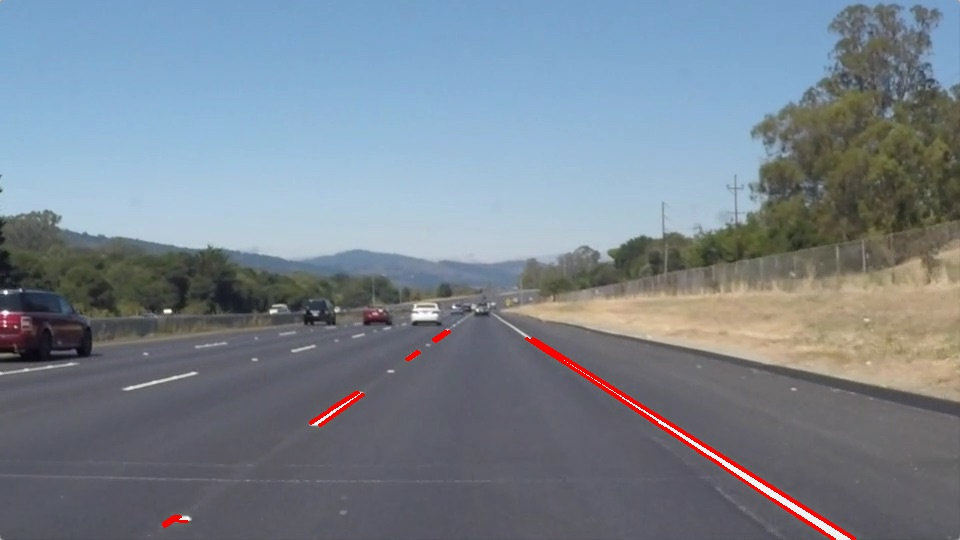
\includegraphics[width=.9\linewidth]{./examples/line-segments-example.jpg}
\caption{\label{fig:org37c61f4}
Example for finding the lane lines on the road}
\end{figure}
\section{Step}
\label{sec:orge6e50ef}
\begin{enumerate}
\item convert the image to the grayscale, hence it is easier to find the lanes.
\item add gaussian blur on the grayscale image to make it "smooth".
\item run the canny algorithm on top of the smoothed image to find all the "edge" by calculate the gradient.
\item clip the interesting region, the region that contains useful information.
\item convert the edge image to the hough space to find the lane line, i.e. the straight line that go through these edge points.
\end{enumerate}
\section{Short Coming}
\label{sec:org992f976}
Everything is hard coded so that we may need to tune the parameters for every single set of road image.
\section{Improvements}
\label{sec:orgd49c568}
Collecting a dataset with labeled lane lines and build an algorithm to auto fit the parameters instead of manually tune it every single time.
\end{document}
